\chapter{Исследовательская часть}

В данном разделе представлены технические характеристики устройства, использованного для измерения времени работы программного обеспечения, а также приведены результаты проведенных замеров.


\section{Технические характеристики}
Характеристики используемого оборудования:
\begin{itemize}
    \item[---] операционная система --- macOS Sequoia 15.1~\cite{macos-sequoia};
    \item[---] память --- 16 Гб;
    \item[---] процессор --- Apple M1 Pro~\cite{apple-silicon}.
\end{itemize}

\section{Постановка задачи}

Цель данного исследования --- установить зависимость времени вставки данных в базу данных от используемого способа добавления данных.

В качестве объекта исследования была выбрана сущность «снимок», а также определены следующие методы вставки данных:

\begin{enumerate}
    \item Постепенная вставка. Реализация данного запроса представлена в листинге~\ref{lst:ins_by_one}.
    \item Пакетная вставка VALUES. Реализация данного запроса представлена в листинге~\ref{lst:ins_by_values}.
    \item Массовая загрузка через COPY. Реализация данного запроса представлена в листинге~\ref{lst:ins_by_copy}.
\end{enumerate}

\begin{center}
\captionsetup{justification=raggedright,singlelinecheck=off}
\begin{lstlisting}[label=lst:ins_by_one, caption=Постепенная вставка]
async fn insert_snap(&self, snap: &Snap) -> Result<(), DataAccessError> {
    let datetime = NaiveDateTime::parse_from_str(
        &format!("{} {}", snap.date, snap.time),
        "%d.%m.%Y %H:%M",
    )
    .map_err(|e| {
        log::error!("Failed to parse datetime: {}", e);
        DataAccessError::InvalidInput(e.to_string())
    })?;

    let query = "INSERT INTO CarSnapshot 
                (camera_id, speed, snap_datetime, gos_num) 
                VALUES ($1, $2, $3, $4)";

    sqlx::query(query)
        .bind(snap.camera.id as i32)
        .bind(snap.speed.map(|s| s as i32))
        .bind(datetime)
        .bind(&snap.gos_num)
        .execute(&self.pool)
        .await
        .map_err(|e| {
            log::error!("Failed to insert snap: {}", e);
            DataAccessError::PsqlDataBaseError(e)
        })?;
    
    Ok(())
}

pub async fn insert_snaps_by_one(&self, snaps: &[Snap]) -> Result<Duration, DataAccessError> {
    let start_time = Instant::now();

    for (i, snap) in snaps.iter().enumerate() {
        let snap_start = Instant::now();
        self.insert_snap(snap).await?;
        log::debug!(
            "Inserted snap {}/{} in {}ms",
            i + 1,
            snaps.len(),
            snap_start.elapsed().as_millis()
        );
    }

    let total_time = start_time.elapsed();
    Ok(total_time)
}
\end{lstlisting}
\end{center}

\begin{center}
\captionsetup{justification=raggedright,singlelinecheck=off}
\begin{lstlisting}[label=lst:ins_by_values, caption=Пакетная вставка VALUES]
pub async fn insert_snaps_by_values(
    &self,
    snaps: &[Snap],
) -> Result<Duration, DataAccessError> {
    let start_time = std::time::Instant::now();

    for chunk in snaps.chunks(100) {
        let mut query_builder = QueryBuilder::new(
            "INSERT INTO CarSnapshot (camera_id, speed, snap_datetime, gos_num) ",
        );

        query_builder.push_values(chunk, |mut b, snap| {
            let datetime = NaiveDateTime::parse_from_str(
                &format!("{} {}", snap.date, snap.time),
                "%d.%m.%Y %H:%M",
            )
            .expect("Failed to parse datetime");

            b.push_bind(snap.camera.id as i32)
                .push_bind(snap.speed.map(|s| s as i32))
                .push_bind(datetime)
                .push_bind(&snap.gos_num);
        });

        let query = query_builder.build();

        query.execute(&self.pool).await.map_err(|e| {
            log::error!("Failed to execute bulk insert: {}", e);
            DataAccessError::PsqlDataBaseError(e)
        })?;
    }

    let total_time = start_time.elapsed();
    Ok(total_time)
}
\end{lstlisting}
\end{center}

\begin{center}
\captionsetup{justification=raggedright,singlelinecheck=off}
\begin{lstlisting}[label=lst:ins_by_copy, caption=Массовая загрузка через COPY]
pub async fn insert_snaps_by_copy(&self, snaps: &[Snap]) -> Result<Duration, DataAccessError> {
    let start_time = std::time::Instant::now();

    let mut connection = self.pool.acquire().await.map_err(|e| {
        log::error!("Failed to acquire connection: {}", e);
        DataAccessError::PsqlDataBaseError(e)
    })?;

    let pg_conn: &mut sqlx::PgConnection = &mut *connection;

    let mut bytes = Vec::new();
    for snap in snaps {
        let datetime = NaiveDateTime::parse_from_str(
            &format!("{} {}", snap.date, snap.time),
            "%d.%m.%Y %H:%M",
        )
        .map_err(|e| {
            log::error!("Failed to parse datetime: {}", e);
            DataAccessError::InvalidInput(e.to_string())
        })?;

        let line = format!(
            "{}\t{}\t{}\t{}\n",
            snap.camera.id,
            snap.speed
                .map(|s| s.to_string())
                .unwrap_or("\\N".to_string()),
            datetime.format("%Y-%m-%d %H:%M:%S"),
            snap.gos_num
        );
        bytes.extend_from_slice(line.as_bytes());
    }

    {
        let mut copy = pg_conn
            .copy_in_raw(
                "COPY CarSnapshot (camera_id, speed, snap_datetime, gos_num) FROM STDIN",
            )
            .await
            .map_err(|e| {
                log::error!("Failed to start COPY: {}", e);
                DataAccessError::PsqlDataBaseError(e)
            })?;

        copy.send(bytes).await.map_err(|e| {
            log::error!("Failed to send COPY data: {}", e);
            DataAccessError::PsqlDataBaseError(e)
        })?;

        copy.finish().await.map_err(|e| {
            log::error!("Failed to finish COPY: {}", e);
            DataAccessError::PsqlDataBaseError(e)
        })?;
    }

    let total_time = start_time.elapsed();
    Ok(total_time)
}
\end{lstlisting}
\end{center}

\section{Результаты замеров}

Каждое значение получено путем взятия среднего из 10 измерений. Зависимость времени вставки от количества вставляемых строк представлена на рисунке~\ref{fig:time_mes}.

\begin{figure}[H]
    \centering
    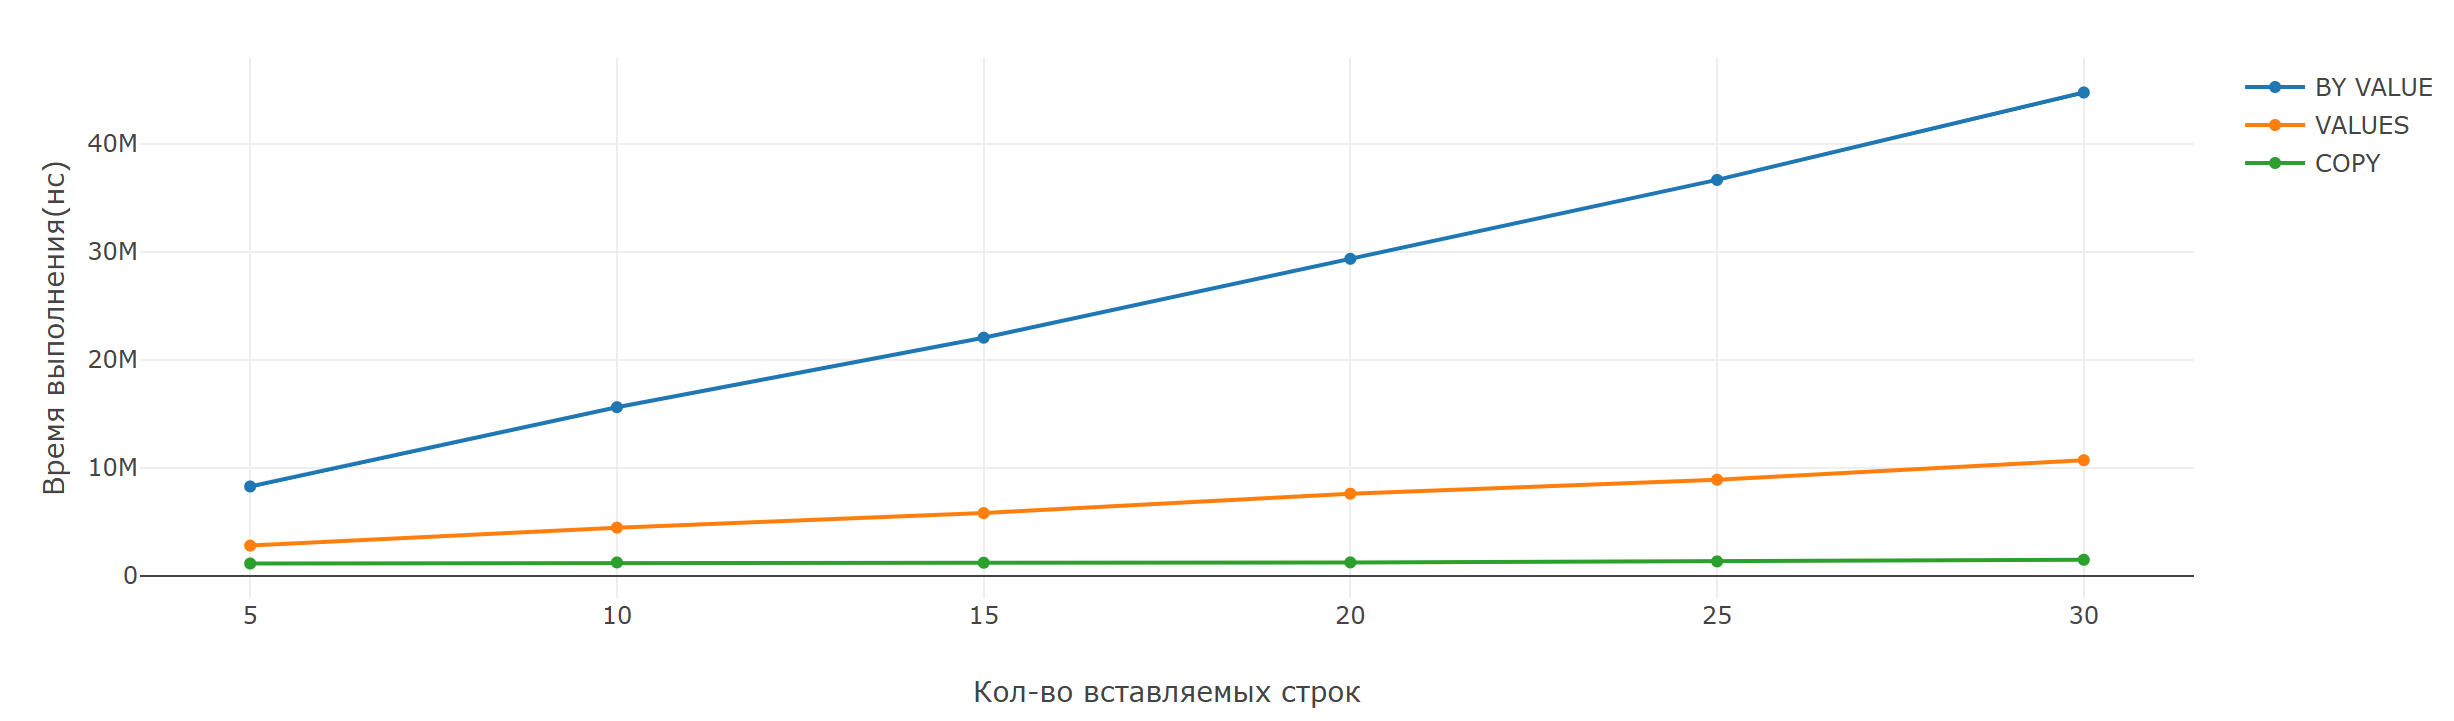
\includegraphics[width=1\linewidth]{images/plots/mes.png}
    \caption{Зависимость времени вставки от количества вставляемых строк}
    \label{fig:time_mes}
\end{figure}


\section{Результат исследования}

На основании проведённого исследования можно сделать вывод, что метод вставки 3 является самым быстрым: при большом объёме вставляемых данных он демонстрирует производительность, превышающую метод 1 более чем в 10 раз, а метод 2 — более чем в 4 раза.

\paragraph*{ВЫВОД} ${}$ \\

В данном разделе рассмотрены технические характеристики устройства, на котором осуществлялось измерение времени работы программного обеспечения, а также представлены полученные результаты замеров.

